\chapter{Wo steckt die zweite L"osung?\label{chapter:komplex}}
\lhead{Bessel-Funktionen zweiter Art}
\begin{refsection}
\chapterauthor{Stefan Kull und Roy Seitz}

\newcommand*\sk{\vcenter{\hbox{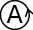
\includegraphics[scale=0.4]{komplex/SK_operator.pdf}}}}

\section{Einleitung}

In diesem Kapitel möchten wir ein Problem aufgreifen, welches wir bei der Bessel'schen Differentialgleichung
\[ z^2w''+zw'+(z^2 - \nu^2)w=0\]
angetroffen haben. 
Wir fanden Lösungen in Form der verallgemeinerten Potenzreihe
\[J_\nu(z)=z^\varrho\sum_{k=0}^{\infty}a_kz^k,\]
und die Indexgleichung lieferte die dazugehörigen $\varrho=\pm\nu.$

\begin{problem*} 
 Eine Differentialgleichung 2. Ordnung besitzt genau zwei linear unabhängige Lösungen.
 Bei $\nu=0$ erhielten wir nur eine Lösung (da $\varrho=0$), und bei ganzzahligen $\nu\in\mathbb{Z}$ besteht eine lineare Abhängigkeit
 \[\nu(z) = J_{-\nu}(-z)\forall\nu\in\mathbb{Z}.\]

Wo also steckt die zweite Lösung?
\end{problem*} 

Dieses Kapitel benötigt zwei bereits beschriebene Werkzeuge, die im Folgenden kurz zusammengefasst sind -- die analytischen Fortsetzung und die Laurent-Reihen.
Anschliessend sollen diese Werkzeuge mit der linearen Algebra kombiniert werden, welches den zentralen Teil dieses Kapitels ausmacht, und abschliessend möchten die Lösungen formell noch gefunden werden.

\subsection{Analytische Fortsetzung}
Die analytische Fortsetzung wurde im Kapitel \ref{sec:fortsetzung} bereits sehr ausführlich Diskutiert.
Die wichtigsten Eigenschaften für die folgende Diskussion seien hier kurz zusammengefasst.

Am Beispiel der Gleichung $y'=\frac{1}{z}$ wurde gezeigt, dass eine Lösung sich bei der analytischen Fortsetzung um eine Singularität verändern kann.
Dies passiert jedoch nur bei mehrdeutigen komplexen Funktionen, also beim Logarithmus und bei Wurzelfunktionen.
Wurzelfunktionen sind hier nicht von Interesse und werden nicht weiter betrachtet. 

Die Veränderung des Logarithmus ist jedoch von zentraler Wichtigkeit.
Abbildung \ref{komplex:analytische-fortsetzung-log} auf Seite \pageref{komplex:analytische-fortsetzung-log} illustriert diese Veränderung.
Bekanntlich ist der Logarithmus nur bis auf ein vielfaches von $2\pi i$ bestimmt. Dies zeigt sich in der analytischen Fortsetzung durch die $2\pi i$, welche beim einmaligen Umlaufen der Singularität hinzukommen.
Durch mehrmaliges Umlaufen des Nullpunktes kann jede Lösung des Logarithmus erreicht werden.

Die analytische Fortsetzung $f^+$ einer Funktion $f$ entlang eines geschlossenen Weges $\gamma$ in positiver Drehrichtung um den Nullpunkt wird in diesem Kapitel sehr oft verwendet.
Wir definieren deshalb den Seitz-Kull-Operator:
\[\sk f(z)= f^+(z)\]
Er soll folgendermassen verstanden werden: wenn man $f(z)$ einmal entlang eines geschlossenen Weges um den Nullpunk in positiver Drehrichtung analytisch fortsetzt, resultiert $f^+(z)$.
Kurz: die analytische Fortsetzung von $f(z)$ ist gleich $f^+(z)$.
Somit lässt sich schreiben: 
\[\sk \log z = \log z + 2\pi i.\]

\subsection{Laurent-Reihe}
Im Kapitel Wegintegrale (\ref{subsection:wegintegrale}) wurde gezeigt, dass eine Funktion $f(z)$ mit einer Singularität nicht in eine Potenzreihe mit ausschliesslich positiven Exponenten entwickelt werden kann.
Auf Seite \pageref{sssec:LaurentReihen} wurde deshalb die Laurent-Reihe hergeleitet, um auch solche Funktionen in Potenzreihen entwickeln zu können.
Da auch Laurent-Reihen in diesem Kapitel mehrfach verwendet werden, soll
\[\mathcal{L}(z):=\sum_{k=-\infty}^{\infty}a_k(z-z_0)^k\]
als Kurzschreibweise für eine Laurent-Reihe im Punkt $z_0$ dienen. Die Stelle $z_0$ wird dabei nicht angegeben, da sie auf die Analyse keinen Einfluss hat.

Laurent-Reihen als Summe ganzzahliger Potenzen sind immer eindeutig.
Die analytische Fortsetzung einer Laurent-Reihe führt folglich wieder auf dieselbe Laurent-Reihe.
Es gilt
\[\sk \mathcal{L}(z)=\mathcal{L}^+(z)=\mathcal{L}(z).\]
Eine Funktion ist also genau dann als Laurent-Reihe darstellbar, wenn sie sich durch die analytische Fortsetzung nicht verändert.

\section{Lineare Algebra}
Die wichtigsten Überlegungen um die zweite linear unabhängige Lösung einer Differentialgleichung 2. Ordnung zu finden, liefert die lineare Algebra.
Wir wissen, dass es zwei linear unabhängige Lösungen geben muss.
Wenn diese Lösungen existieren, dann können sie auch analytisch fortgesetzt werden.
Im Folgenden sei $w$ der Vektor der beiden linear unabhängigen Lösungen
\[w = \begin{pmatrix} w_1 \\ w_2 \end{pmatrix} \]
und $w^+$ die analytische Fortsetzung dieser Lösungen
\[w^+= \sk w = \begin{pmatrix}
w_1^+\\ w_2^+
\end{pmatrix}.
\]
Da es insgesammt nur zwei linear unabhängige Lösungen geben kann, muss zwischen $w$ und $w^+$ eine lineare Abhängigkeit bestehen.
Es existiert also eine Matrix
\[A = \begin{pmatrix}a_{11} & a_{12} \\ a_{21} & a_{22}\end{pmatrix}\]
so das gilt
\[\sk w = w^+ = Aw.\]
Die analytische Fortsetzung kann also durch die Matrix $A$ beschrieben werden.

Aus der linearen Algebra ist bekannt, dass für \emph{reguläre} Matrizen durch geeignete Transformation immer eine Basis gefunden werden kann, in welcher $A$ entweder Diagonalform oder Dreiecksform besitzt.
Die Diagonalform kann erreicht werden, wenn die Matrix $A$ zwei verschiedene Eigenwerte $\lambda_1$ und $\lambda_2$ besitzt. 
\[A'=\begin{pmatrix}
\lambda_1 & 0 \\ 
0 & \lambda_2 \end{pmatrix}\]
Sind die beiden Eigenwerte gleich, also im Falle $\lambda_1=\lambda_2=\lambda$, lässt sich die Matrix möglicherweise nicht diagonalisieren, bestimmt jedoch auf die Dreiecksform
\[A'=\begin{pmatrix}\lambda & 0 \\ 1 & \lambda\end{pmatrix}\]
reduzieren.

Zunächst ist jedoch ein Beweis vonnöten, dass die analytische Fortsetzung linear unabhängiger Lösungen wiederum auf linear unabhängige Lösungen führt, die Matrix $A$ also regulär ist.
Wäre die Matrix $A$ singulär, liesse sich auch die Zerlegung in Diagonal- oder Dreiecksform nicht durchführen. 

\subsection{Beweis der Regularität von $A$}
Eine Konstante kann als Spezialfall einer Laurent-Reihe betrachtet werden
\[c = \mathcal{L}_1(z)=\sum_{k=-\infty}^{\infty}a_k(z-z_0)^k\qquad\text{wobei}\qquad  z_0=0, a_k=\begin{cases}
c&k=0\\0&\text{sonst}
\end{cases}\]
Somit ist die analytische Fortsetzung einer Funktion genau dann konstant, wenn die Funktion selbst konstant ist.
\[c = \mathcal{L}_1(z)= \sk \mathcal{L}_1(z) = \sk c.\]
$w_1$ und $w_2$ sind linear unabhängig. Deren Verhältnis ist also nicht konstant
\[w_1\ne a w_2\quad\Rightarrow\quad\frac{w_1}{w_2}\ne a.\]
Die analytische Fortsetzung diese Verhältnisses ist folglich auch nicht konstant
\[\frac{w_1^+}{w_2^+}=\sk \left(\frac{w_1}{w_2}\right) \ne \sk a = a \]
\[\Rightarrow\quad \frac{w_1^+}{w_2^+}\ne a\quad\Rightarrow\quad w_1^+\ne aw_2^+\qed
\]

Die analytische Fortsetzung linear unabhängiger Lösungen $w$ führt also stets auf wiederum linear unabhängige Lösungen $w^+$.
Die Matrix $A$ ist also in jedem Falle regulär und lässt sich durch Wahl zweier geeigneter Lösungen $w_1$ und $w_2$ für jede Differentialgleichung 2. Ordnung entweder in Diagonal- oder Dreiecksform zerlegen.
Diese beiden Fälle werden nun diskutiert.



\hyphenation{werden Nenner einfacher Summe weiteren welcher verwendet angegeben Index-gleichung zusammen-gefasst Koeffizient Koeffizienten Differential-gleichung Klammer Spezial-fall Problems be-kommen}
\section[Potenzreihenherleitung der Besselfunktion]{Potenzreihenherleitung der Besselfunktion 1. Art}
\begin{normalsize}
Im vorhergehenden Abschnitt wurde die Besselsche Differentialgleichung \refeq{eq:besselsche_dgl} hergeleitet.
Um diese zu l\"osen wird $\mu = - 1$ gesetzt und das Vorzeichen vor der Klammer gekehrt
\end{normalsize}
\begin{align}
	r^2 \, R'' \left( r \right)
	+
	r \, R' \left( r \right)
	+
	\big( r^2 - n^2 \big) \, R \left( r \right)
	=
	0
	\label{eq:bessel:dgl}
	\text{.}
\end{align}
\begin{normalsize}%
Durch die Vereinfachung $\mu = -1$ ist die Differentialgleichung \refeq{eq:bessel:dgl} nur durch eine Skalierung von der Differentialgleichung \refeq{eq:besselsche_dgl} verschieden.
Zum L\"osen der Differentialgleichung \refeq{eq:bessel:dgl} wird die Potenzreihen-Methode aus dem Kapitel \ref{section:potenzreihen:verallgemeinert} verwendet.
\end{normalsize}
\subsection{Vorgehensweise f\"ur die Herleitung der Besselfunktion}
\begin{normalsize}%
Die Herleitung der Besselfunktion beinhaltet folgende Schritte:
\end{normalsize}
\begin{compactenum}
	\item Die Potenzreihe und deren Ableitungen berechnen.
	\item Die Potenzreihen in die Differentialgleichung \refeq{eq:bessel:dgl} einsetzen, um \dots
	\item die Indexgleichung f\"ur $\varrho$ zu l\"osen, welche \dots
	\item \dots eine Rekursion der Koeffizienten erm\"oglicht.
	\item Bestimmen der Koeffizienten f\"ur \dots
	\item \dots die Besselfunktion mit ganzzahligen Parametern \refeq{eq:bessel:summenformel}.
%	\item Allgemeine Besselfunktion \refeq{eq:bessel_summenformel:allgemein}
\end{compactenum}
\newcounter{stepCounter}
\setcounter{stepCounter}{1}
\subsubsection{\arabic{stepCounter}. Schritt: Potenzreihe und deren Ableitungen berechnen}
\stepcounter{stepCounter}
\begin{normalsize}
Wie schon erw\"ahnt,
kann mit Hilfe der Potenzreihen-Methode die Differentialgleichung \refeq{eq:bessel:dgl} gel\"ost werden.
F\"ur den Ansatz ben\"otigen wir zuerst eine verallgemeinerte Potenzreihe
\end{normalsize}
\begin{align}
	R \left( r \right)
	&=
	r^{\varrho}
	\sum_{k=0}^{\infty} a_k \, r^k .
	\label{eq:bessel:potenzreihe:verallgemeinert}
\end{align}
\begin{normalsize}%
Da in der Differentialgleichung die erste und zweite Ableitung vorkommt,
muss die Potenzreihe abgeleitet werden,
\end{normalsize}
\begin{align}
	R'\left( r \right)
	&=
	\varrho \, r^{\varrho - 1}
	\sum_{k=0}^{\infty} a_k \, r^k
	+
	r^{\varrho}
	\sum_{k=0}^{\infty} a_k \, k \, r^{k - 1}
	\label{eq:bessel:potenzreihe:ersteableitung}
\\
	R'' \left( r \right)
	&=
	\varrho \, \left( \varrho - 1 \right) \, r^{\varrho - 2}
	\sum_{k=0}^{\infty} a_k \, r^k
	+
	2 \, \varrho \, r^{\varrho - 1}
	\sum_{k=0}^{\infty} a_k \, k \, r^{k - 1}
	+
	r^{\varrho}
	\sum_{k=0}^{\infty} a_k \, k \, \left( k - 1 \right) \, r^{k - 2}	
	\label{eq:bessel:potenzreihe:zweiteableitung}
	\text{,}
\end{align}
\begin{normalsize}%
was wiederum eine Potenzreihe ergibt.
\end{normalsize}
\subsubsection{\arabic{stepCounter}. Schritt: Potenzreihen in Differentialgleichung \refeq{eq:bessel:dgl} einsetzen}
\stepcounter{stepCounter}
\begin{normalsize}%
Als n\"achstes werden die erhaltenen Potenzreihen in die Differentialgleichung
\end{normalsize}
\begin{align*}
	\textcolor{mygreen}{r^2 \, R'' \left( r \right)}
	+
	\textcolor{teal}{r \, R' \left( r \right)}
	+
	\textcolor{blue}{\big( r^2 - n^2 \big) \, R \left( r \right)}
	=
	0
	\tag{\ref{eq:bessel:dgl}}
\end{align*}
\begin{normalsize}%
eingesetzt \dots
\end{normalsize}
\begin{align*}	
	\textcolor{mygreen}{
		\varrho \, \left( \varrho - 1 \right) \, r^{\varrho}
		\sum_{k=0}^{\infty} a_k \, r^k
		+
		2 \, \varrho \, r^{\varrho}
		\sum_{k=0}^{\infty} a_k \, k \, r^k
		+
		r^{\varrho}
		\sum_{k=0}^{\infty} a_k \, k \, \left( k - 1 \right) \, r^k
	}
	+ \\
	\textcolor{teal}{
		\varrho \, r^{\varrho}
		\sum_{k=0}^{\infty} a_k \, r^k
		+
		r^{\varrho}
		\sum_{k=0}^{\infty} a_k \, k \, r^k
	}
	+ 
	\textcolor{blue}{
		\big(
		r^2 - n^2
		\big) \,
		r^{\varrho}
		\sum_{k=0}^{\infty} a_k \, r^k
	}
	= & \, 0
\end{align*}
\begin{normalsize}%
\dots , ausmultipliziert \dots
\end{normalsize}
\begin{align*}
	\textcolor{mygreen}{	\varrho \, \left( \varrho - 1 \right)} 
	\, r^{\varrho}
	\sum_{k=0}^{\infty} a_k \, r^k
	+
	\textcolor{mygreen}{2 \, \varrho}
	\, r^{\varrho}
	\sum_{k=0}^{\infty} a_k \, k \, r^k
	+
	r^{\varrho}
	\sum_{k=0}^{\infty} a_k \, k \, \left( k - 1 \right) \, r^k
	+ \\
	\textcolor{teal}{\varrho}
	\, r^{\varrho}
	\sum_{k=0}^{\infty} a_k \, r^k
	+
	r^{\varrho}
	\sum_{k=0}^{\infty} a_k \, k \, r^k
	+
	r^{\varrho}
		\sum_{k=0}^{\infty} a_k \, r^{k \textcolor{blue}{+ 2}}
	-
	\textcolor{blue}{n^2}
	\, r^{\varrho}
	\sum_{k=0}^{\infty} a_k \, r^k
	= & \, 0
\end{align*}
\begin{normalsize}%
\dots und die Terme mit der gleichen Potenz von $r$ zusammengefasst
\end{normalsize}
\begin{align}
	\big(
	\textcolor{mygreen}{\varrho \, \left( \varrho - 1 \right)}
	+ 
	\textcolor{teal}{\varrho}
	-
	\textcolor{blue}{n^2}
	\big)
	\, r^{\varrho}
	\sum_{k=0}^{\infty} a_k \, r^k
	+ 
	\left(
	\textcolor{mygreen}{2 \, \varrho}
	+
	\textcolor{teal}{1}
	\right)
	\, r^{\varrho}
	\sum_{k=0}^{\infty} a_k \, k \, r^k
	+
	r^{\varrho}
	\sum_{k=0}^{\infty} a_k \, k \, \left( k - 1 \right) \, r^k
	+ 
	r^{\varrho}
	\sum_{k=0}^{\infty} a_k \, r^{k + 2}
	= \, 0
	\label{eq:bessel:potenzreihe:dgl:vereinfacht}
	\text{.}
\end{align}
%\begin{normalsize}%
%Die resultierende Gleichung \refeq{eq:bessel:potenzreihe:dgl:vereinfacht} sieht auf den ersten Blick komplizierter aus,
%als die urspr\"ungliche Differentialgleichung \refeq{eq:bessel:dgl}.
%\end{normalsize}
\subsubsection{\arabic{stepCounter}. Schritt: Indexgleichung zum Bestimmen von $\varrho$}
\stepcounter{stepCounter}
\begin{normalsize}%
Beim Koeffizientenvergleich werden alle Terme,
welche die gleiche Potenz von $r$ haben,
mit $0$ gleichgesetzt,
da die Differentialgleichung f\"ur jede Potenz gelten muss.
Der Koeffizientenvergleich f\"ur die tiefste Potenz (im vorliegenden Fall $\varrho + 0$) wird auch Indexgleichung genannt.
Demzufolge ist die Indexgleichung f\"ur die Gleichung \refeq{eq:bessel:potenzreihe:dgl:vereinfacht}
\end{normalsize}
\begin{align}
	\big( \varrho \, \left( \varrho -1 \right) + \varrho - n^2 \big)
	\, r^{\varrho + 0} \, a_0 &= 0
	\label{eq:bessel:indexgleichung:ausgangslage}
	\text{,}
\end{align}
\begin{normalsize}%
bzw.
\end{normalsize}
\begin{align}
	\big( \varrho \, \left( \varrho -1 \right) + \varrho - n^2 \big) &= 0
	\label{eq:bessel:indexgleichung:ausgangslage:vereinfacht}
	\text{.}
\end{align}
\begin{normalsize}%
In der Indexgleichung \refeq{eq:bessel:indexgleichung:ausgangslage:vereinfacht} hat es nur eine Unbekannte $\varrho$,
nach welcher die Indexgleichung aufgel\"ost werden kann:
\end{normalsize}
\begin{align*}
	\varrho \, \left( \varrho -1 \right) + \varrho - n^2 &= 0 \\
	\varrho ^2 - \varrho + \varrho -n^2 &= 0  \\
	\varrho ^2 - n^2 &= 0 \\
	\varrho ^2 &= n^2 \\
	\varrho &= \pm n
	\text{.}
\end{align*}
\begin{normalsize}%
Da die Indexgleichung eine quadratische Gleichung ist,
muss es immer zwei L\"osungen geben,
was bis auf den Fall $n = 0$ erf\"ullt ist.
Wie die zweite L\"osung f\"ur den Fall $n = 0$ bzw. $\varrho = 0$ zustande kommt,
wird im Kapitel \ref{chapter:Loesung2} genauer erkl\"art.
\end{normalsize}
\subsubsection{\arabic{stepCounter}. Schritt: Rekursion der Koeffizienten $a_k$}
\stepcounter{stepCounter}
\begin{normalsize}%
Die Indexgleichung ergibt, dass $n$ f\"ur $\varrho$ in der Gleichung \refeq{eq:bessel:potenzreihe:dgl:vereinfacht} eingesetzt werden kann:
\end{normalsize}
\begin{align}
	\big(
	n \, \left( n - 1 \right)
	+
	n
	-
	n^2
	\big)
	\, r^{n}
	\sum_{k=0}^{\infty} a_k \, r^k
	+
	\left(	
	2 \, n
	+
	1
	\right)
	\, r^{n}
	\sum_{k=0}^{\infty} a_k \, k \, r^k
	+
	r^{n}
	\sum_{k=0}^{\infty} a_k \, k \, \left( k - 1 \right) \, r^k
	+
	r^{n}
	\sum_{k=0}^{\infty} a_k \, r^{k + 2}
	= \, 0
	\label{eq:bessel:potenzreihe:dgl:index:eingesetzt}
	\text{.}
\end{align}
\begin{normalsize}%
%Da bekanntlich nur Terme mit der gleichen Potenz miteinander verrechnet werden k\"onnen,
F\"ur einen Koeffizientenvergleich sollen alle Summen in der Gleichung \refeq{eq:bessel:potenzreihe:dgl:index:eingesetzt} so umgeformt werden,
dass sie den Term $r^k$ enthalten.
Eine Summe enth\"alt den Term $r^{k + 2}$,
welcher auf $r^k$ umgeformt werden muss.
Dazu wird der Start-Index der Summe von $k = 0$ auf $k = 2$ ge\"andert und alle $k$'s in der Summe durch $k - 2$ ersetzt.
Nun haben alle Summen den Term $r^k$ enthalten
\end{normalsize}
\begin{align}
	\big(
	n \, \left( n - 1 \right)
	+
	n
	-
	n^2
	\big)
	\, r^{n}
	\sum_{k=0}^{\infty} a_k \, r^k
	+
	\left(	
	2 \, n
	+
	1
	\right)
	\, r^{n}
	\sum_{k=0}^{\infty} a_k \, k \, r^k
	+
	r^{n}
	\sum_{k=0}^{\infty} a_k \, k \, \left( k - 1 \right) \, r^k
	+
	r^{n}
	\sum_{k=2}^{\infty} a_{k - 2} \, r^k
	= \, 0
	\label{eq:bessel:potenzreihe:dgl:index:eingesetzt:gleichesummen}
	\text{.}
\end{align}
\begin{normalsize}%
In der Gleichung \refeq{eq:bessel:potenzreihe:dgl:index:eingesetzt:gleichesummen} k\"onnen die einzelnen Summen zu einer einzigen Summen zusammengefasst werden.
Allerdings haben die Summen unterschiedliche Startindizes.
Die einen Summen haben als Start-Index $k = 0$,
wobei die andere Summe einen Start-Index von $k = 2$ hat.
%Damit die Summen trotzdem zusammengefasst werden k\"onnen,
%werden die Terme mit dem Index $k < 2$ weggelassen.
Durch die Indexgleichung kann sichergestellt werden,
dass die Koeffizienten f\"ur $k < 2$ wegfallen,
bzw. 0 sind.
Somit darf als Start-Index $k = 2$ verwendet werden.
\end{normalsize}
\begin{align}
	r^n
	\sum_{k=2}^{\infty}
	\biggl(
	n \, \left( n - 1 \right) \, a_k 
	+
	2 \, n \, k \, a_k
	+
	k \, \left( k - 1 \right) \, a_k
	+
	n \, a_k
	+
	k \, a_k
	+
	a_{k - 2}
	-
	n^2 \, a_k
	\biggr)
	\, r^k
	= 0 
	\label{eq:bessel:summe:zusammengefasst}
	\\
	\nonumber
	r^n
	\sum_{k=2}^{\infty}
	\biggl(
	\left( n^2 - \, n \right) \, a_k 
	+
	2 \, n \, k \, a_k
	+
	\left( k^2 - \, k \right) \, a_k
	+
	n \, a_k
	+
	k \, a_k
	+
	a_{k - 2}
	-
	n^2 \, a_k
	\biggr)
	\, r^k
	= 0 
	\\
	\nonumber
	r^n
	\sum_{k=2}^{\infty}
	\biggl(
	\left( n^2 - \, n \right) \, a_k 
	-
	n^2 \, a_k
	+
	n \, a_k
	+
	\left( k^2 - \, k \right) \, a_k
	+
	k \, a_k
	+
	2 \, n \, k \, a_k
	+
	a_{k - 2}
	\biggr)
	\, r^k
	= 0 
	\\
	\nonumber
	r^n
	\sum_{k=2}^{\infty}
	\biggl(
	\left( n^2 - n \right) \, a_k 
	-
	n^2 \, a_k
	+
	n \, a_k
	+
	k^2 \, a_k
	+
	2 \, n \, k \, a_k
	+
	a_{k - 2}
	\biggr)
	\, r^k
	= 0 
	\\
	\nonumber
	r^n
	\sum_{k=2}^{\infty}
	\biggl(
	n^2 \, a_k 
	-
	n^2 \, a_k
	+
	k^2 \, a_k
	+
	2 \, n \, k \, a_k
	+
	a_{k - 2}
	\biggr)
	\, r^k
	= 0 
	\\
	r^n
	\sum_{k=2}^{\infty}
	\biggl(
	k^2 \, a_k
	+
	2 \, n \, k \, a_k
	+
	a_{k - 2}
	\biggr)
	\, r^k
	= 0
	\label{eq:bessel:summe:zusammengefasst:vereinfacht}
\end{align}
\begin{normalsize}%
%Die Gleichung \refeq{eq:bessel:summe:zusammengefasst} kann durch einfache Rechnungsschritte zu der Gleichung \refeq{eq:bessel:summe:zusammengefasst:vereinfacht} umgeformt werden.
Die Gleichung \refeq{eq:bessel:summe:zusammengefasst:vereinfacht} besagt,
dass $r$ oder die Summe $0$ ergeben muss.
$r = 0$ ist dabei ein Spezialfall, welcher keine Rekursion der Koeffizienten erm\"oglicht und somit nicht zur L\"osung des Problems f\"uhrt.
Demzufolge muss die Summe, bzw. die Klammer, $0$ ergeben.
Wird der Ausdruck in der Klammer,
aus der Gleichung
\end{normalsize}
\begin{align*}
	r^n
	\sum_{k=2}^{\infty}
	\biggl(
	k^2 \, a_k
	+
	2 \, n \, k \, a_k
	+
	a_{k - 2}
	\biggr)
	\, r^k
	= 0
	\tag{\ref{eq:bessel:summe:zusammengefasst:vereinfacht}}
	\text{,}
\end{align*}
\begin{normalsize}%
mit $0$ gleichgesetzt
\end{normalsize}
\begin{align*}
	2 \, n \, k \, a_k
	+
	k^2 \, a_k
	+
	a_{k - 2}
	= 0
\end{align*}
\begin{normalsize}
und nach dem Koeffizient $a_k$ aufgel\"ost
\end{normalsize}
\begin{align}
	\nonumber
	\big(
	2 \, n \, k 
	+
	k^2 
	\big)
	\, a_k
	+
	a_{k - 2}
	= 0 
	\\
	\nonumber
	k \,
	\big(
	2 \, n
	+
	k
	\big)
	\, a_k
	= -a_{k - 2}
	\\
	a_k
	=
	\frac
	{
		-a_{k - 2}
	}{
		k \, \left( 2 \, n + k \right)	
	}
	\label{eq:bessel:koeffizienten:rekursion}
	\text{,}
\end{align}
\begin{normalsize}
kann eine Rekursion der Koeffizienten gefunden werden.
\end{normalsize}
\subsubsection{\arabic{stepCounter}. Schritt: Bestimmen der Koeffizienten $a_k$ mit Hilfe der Rekursionsformel \refeq{eq:bessel:koeffizienten:rekursion}}
\stepcounter{stepCounter}
\begin{normalsize}%
Die Rekursionsformel \refeq{eq:bessel:koeffizienten:rekursion} besagt,
dass der Koeffizient $a_k$ vom Koeffizient $a_{k-2}$ linear abh\"angt.
Somit sind alle geraden Koeffizienten linear von $a_0$ abh\"angig und alle un\-geraden Koeffizienten von $a_1$.
Da aber laut der Rekursionsformel \refeq{eq:bessel:koeffizienten:rekursion} $a_1$ aus $a_{-1}$ berechnet werden kann und $a_{-1} = 0$ ist,
entfallen alle ungeraden Koeffizienten.
Damit nur mit den geraden Koeffizienten gerechnet wird,
wird $k$ durch $2k$ in der Rekursionsformel \refeq{eq:bessel:koeffizienten:rekursion} ersetzt
\end{normalsize}
\begin{align}
	\nonumber
	a_{2k}
	&=
	\frac
	{
		-a_{2k - 2}
	}{
		2k \, \left( 2 \, n + 2k \right)	
	}
	=
	\frac
	{
		-a_{2k - 2}
	}{
		4k \, \left( n + k \right)	
	}
	\text{.}
\end{align}
\begin{normalsize}%
Um den Koeffizienten $a_{2k}$ zu berechnen,
muss zuerst der Koeffizient $a_{2k-2}$ berechent werden,
welcher aus dem Koeffizienten $a_{2k-2-2}$ berechnet wird.
F\"ur den Koeffizient $a_{2k}$ m\"ussen demzufolge alle Koeffizienten zwischen $a_0$ und $a_{2k}$ bekannt sein.
Diese Berechnung ist sehr Zeit und Rechenintesiv.
Daher wird nach einer Formel f\"ur $a_{2k}$ gesucht,
wo der Koeffizient $a_{2k}$ direkt aus dem Koeffizient $a_0$ mit linearen Operationen berechnet werden kann.
Um eine direkte Formel f\"ur $a_{2k}$ zu bekommen,
hat es sich bew\"ahrt,
die Koeffizienten $a_2$, $a_4$ , $a_6$ , \dots \, zu berechnen,
bis eine Regelm\"assigkeit erkennbar ist.
Die Koeffizienten sehen wiefolgt aus:
\end{normalsize}
\begin{align}
	\nonumber
	a_2
	&=
	\frac
	{
		-a_0
	}{
		4 \, \left( n + 1 \right)	
	}
	\\
	\nonumber
	a_4
	&=
	\frac
	{
		-a_{2}
	}{
		8 \, \left( n + 2 \right)	
	}
	=
	\frac
	{
		- \left( - a_{0} \right)
	}{
		8 \, \left( n + 2 \right) \, 4 \, \left( n + 1 \right)
	}
	=
	\frac
	{
		\left( -1 \right) ^2 \, a_{0}
	}{
		32 \, \left( n + 2 \right) \, \left( n + 1 \right)
	}
	\\
	\nonumber
	a_6
	&=
	\frac
	{
		-a_{4}
	}{
		12 \, \left( n + 3 \right)	
	}
	=
	\frac
	{
		- \left( - a_{2} \right)
	}{
		12 \, \left( n + 3 \right) \, 8 \, \left( n + 2 \right)
	}
	=
	\dots
	=
	\frac
	{
		\left( -1 \right) ^3 \, a_{0}
	}{
		4^3 \, {3}! \, {\left( n + 3 \right)}!
	}
	\\
	\nonumber
	& \, \, \, \vdots
	\\
	a_{2k}
	&=	
	\frac
	{
		\left( -1 \right) ^k \, a_0 
	}{
		4^k \, {k}! \, {\left( n + k \right)}!
	}
	=
	\frac
	{
		\left( -1 \right) ^k \, a_0
	}{
		2^{2k} \, {k}! \, {\left( n + k \right)}!
	}
	\label{eq:bessel:koeffizienten:gerade}
	\text{.}
\end{align}
\subsubsection{\arabic{stepCounter}. Schritt: Besselfunktion f\"ur ganzzahligen Parameter $n$}
\stepcounter{stepCounter}
\begin{normalsize}%
Die Koeffizienten $a_k$ k\"onnen nun in die urspr\"ungliche Potenzreihe \refeq{eq:bessel:potenzreihe:verallgemeinert} eingesetzt werden.
Da bei den Koeffizienten die Indexvariable $k$ durch $2k$ ersetzt wurde,
muss diese \"Anderung auch f\"ur die urspr\"unglichen Potenzreihe \"ubernommen werden
\end{normalsize}
\begin{align}
	R \left( r \right)
	&=
	r^{n} \,
	\sum_{k=0}^{\infty}
	\frac
	{
		\left( -1 \right) ^k \, a_0
	}{
		2^{2k} \, {k}! \, {\left( n + k \right)}!
	}
	\, r^{2k}
	=
	\sum_{k=0}^{\infty}
	\frac
	{
		\left( -1 \right) ^k \, a_0
	}{
		2^{2k} \, {k}! \, {\left( n + k \right)}!
	}
	\, r^{2k + n}
	\label{eq:bessel:potenzreihe:koeffizienten:eingesetzt}
	\text{.}
\end{align}
\begin{normalsize}%
In der Potenzreihe \refeq{eq:bessel:potenzreihe:koeffizienten:eingesetzt} gibt es jedoch den unbekannten Koeffizienten $a_0$,
welcher f\"ur die weiteren Koeffizienten ben\"otigt wird.
Die Variable $r$ in der Potenzreihe \refeq{eq:bessel:potenzreihe:koeffizienten:eingesetzt} hat die Potenz $2k + n$.
Im Nenner kommt bei $2^{2k}$ eine \"ahnliche Potenz vor.
Daher wird nun $a_0 = 2^{-n}$ gew\"ahlt,
um auch im Nenner auf die Potenz $2k + n$ zu kommen.
\end{normalsize}
\begin{align*}
	R \left( r \right)
	&=
	\sum_{k=0}^{\infty}
	\frac
	{
		\left( -1 \right) ^k \, a_0
	}{
		2^{2k} \, {k}! \, {\left( n + k \right)}!
	}
	\, r^{2k + n}
	=
	\sum_{k=0}^{\infty}
	\frac
	{
		\left( -1 \right) ^k
	}{
		2^{2k} \, 2^n \, {k}! \, {\left( n + k \right)}!
	}
	\, r^{2k + n}
	=
	\\
	&=
	\sum_{k=0} ^{\infty}
	\frac
	{
		\left( - 1 \right) ^k \, r ^{2k+n}
	}{
		2^{2k+n} \, {k}! \, { \left( k + n \right) }!
	}
	=
	\sum_{k=0} ^{\infty}
	\frac
	{
		\left( - 1 \right) ^k \, 
		\frac
		{
			r ^{2k+n}
		}{
			2^{2k+n}
		}
	}{
		{k}! \, { \left( k + n \right) }!
	}
	=
	\sum_{k=0} ^{\infty}
	\frac
	{
		\left( - 1 \right) ^k \, 
		\left(		
		\frac
		{
			r
		}{
			2
		} \right) ^{2k+n}
	}{
		{k}! \, { \left( k + n \right) }!
	}
	\text{.}
\end{align*}
\begin{normalsize}%
F\"ur die Besselfunktion wird meist der Buchstabe $J$ verwendet,
wo der Parameter $n$ tiefgestellt angegeben wird.
Die Funtion
\end{normalsize}
\begin{align}
	J_n \left( r \right)
	&=
	\sum_{k=0} ^{\infty}
	\frac
	{
		\left( - 1 \right) ^k \, 
		\left(		
		\frac
		{
			r
		}{
			2
		} \right) ^{2k+n}
	}{
		{k}! \, { \left( k + n \right) }!
	}
	\label{eq:bessel:summenformel}
\end{align}
\begin{normalsize}%
heisst \emph{Bessel-Funktionen} erster Art.
Die Potenzreihe \refeq{eq:bessel:summenformel} ist die L\"osung f\"ur die Differentialgleichung \refeq{eq:bessel:dgl}.
Die Abbildung \ref{img:besselfunction} illustriert die Besselfunktion \refeq{eq:bessel:summenformel} f\"ur ausgew\"ahlte $n$'s.
\end{normalsize}
\begin{figure}[h]
	\begin{center}
		\includegraphics[scale=0.5]{kreis/besselfunction.pdf}
		\caption[Besselfunktion 1. Art]{Darstellung der Besselfunktionen 1. Art}
		\label{img:besselfunction}
	\end{center}
\end{figure}



\printbibliography[heading=subbibliography]
\end{refsection}

